\chapter{Related Work}
\label{Related Work}
This section discusses the most important work found related to the thesis. It starts with mentioning similar techniques with the same goal: Detecting human activity. It then summarises all projects done which use light reach the same goal. This chapter finalises with used in other projects using visible light which can be applied in this thesis.

\section{Related techniques}
Passive localization, the act of sensing the presence of humans or objects which do not actively participate in the process, is a common problem and has been tackled in many different ways by companies and research groups. Several techniques used by these groups will be mentioned here while pointing out what specific ideas could be used to improve the thesis.

M. Youssef \textit{et al.} created a detect and track application with the help of WIFI access-points (APs) and WIFI monitoring-points (MPs) and an aplication sever (AS)\cite{WIFI_Tracking}. The MPs measure the signal strength of the APs, and transmit this data to the AS. The server runs a moving variance algorithm on all of the received signals to detect significant changes in the signal. An overview of the complete system can be seen in figure \ref{fig:WIFI-tracking}.

\begin{figure}[]
	\centering
	\label{fig:WIFI-tracking}
	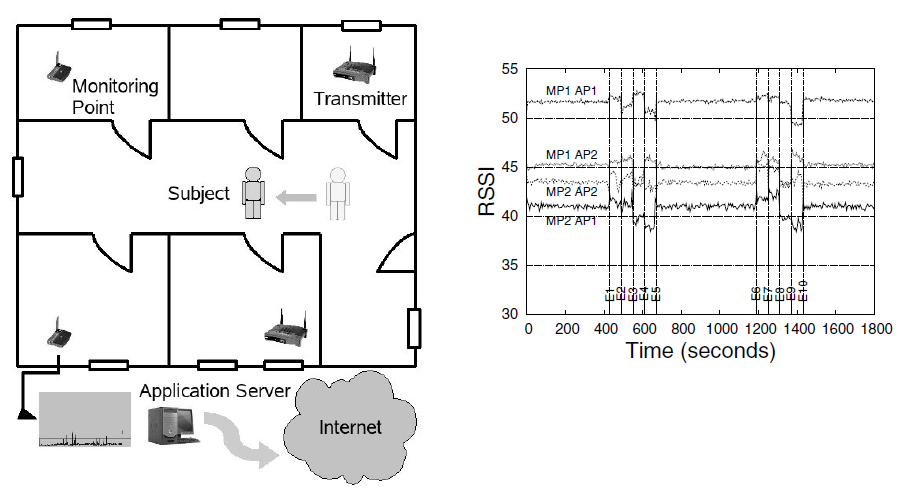
\includegraphics[width=\textwidth]{pics/MovingVarriance1.png}
	\caption{Overview of the WIFI tracking system of Moustsafa Youssef \textit{et al.} \cite{WIFI_Tracking}. The left figure shows an overview of the setup where the right figure shows the strength of the APs from the point of view of the MPs. E1 to E8 represent possible 'events' of bypassing persons.}
\end{figure}

M. Valtonen \textit{et al} created a system which passively tracks humans with the help of capacitive street tiles\cite{Tile_Track}. 
Byunghun Song \textit{et al}\cite{PIR_Tracking}
Smart street light system \cite{tvilight}


\section{Human sensing with visible light}
\label{sec:Visible light communication}
This thesis attempts to solve the passive localization problem with only visible light a luminaire would normally emit and a single light sensor mounted on the ceiling. Several other projects have attempted similar challenges using visible light. E.D. Lascio \textit{et al.} has created a system which uses a ceiling mounted luminaire and light sensors in the floor as seen in figure \ref{fig:LocalLight} \cite{LocaLight}. A human passing by in interrupt the light rays and cast a shadow on the photo diode, resulting in a detection.

T. Li \textit{et al.} takes the concept of lights on the ceiling and photo diodes on the floor to the next level in \cite{Human_Sensing_Using_VLC}. By placing multiple lights on the ceiling and photo diodes on the floor, they create a pixelated image of a person standing from the point of view of each light on the ceiling (see figure \ref{fig:humansensingwithvisiblelight}). These pixel-images are then used to reconstruct the original stance of the person scanned.

\begin{figure}[]
	\centering
	\label{fig:LocalLight}
	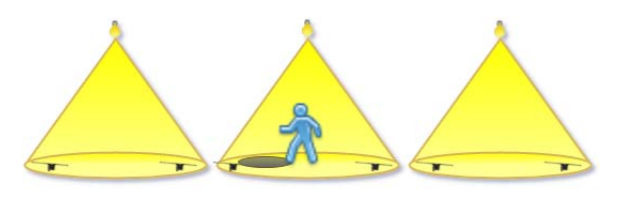
\includegraphics[width=90mm]{pics/LocalLight.png}
	\caption{Overview of the LocalLight system of E.D. Lascio \textit{et al}. Lights on the ceiling and light sensing RFID tags on the floor.}
\end{figure}

\begin{figure}[]
	\centering
	\label{fig:humansensingwithvisiblelight}
	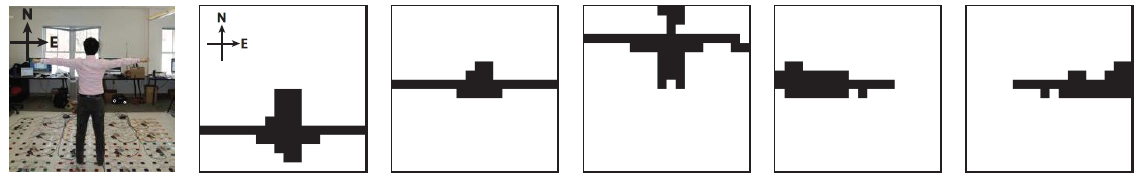
\includegraphics[width=\textwidth]{pics/humansensingwithvisiblelight.png}
	\caption{The scanned person with the resulting created pixel images.}
\end{figure}

C. Zhang \textit{et al} \cite{Near_Field_VLS}

J. Zhang for example created a method for localizing and tracking objects with specular surfaces on a line\cite{JakesWork}. 

Another example of indoor activity detection is the project of M. Ibrahim \textit{et al}. They detect humans or bypassing objects with the help of multiple lights and photo diodes hung at a ceiling\cite{Ceiling_PD}. Normally, if nobody is in the room, all lights shine on the floor, and reflect some rays of light back to each photo diode hanging on the ceiling. If an object passes by which interrupts this light ray, then a shadow is created on the floor. The photo-diode hanging at another light will notice the reduced reflection and a detection is triggered. An overview of this set-up can be seen in figure \ref{fig:Ceiling_PD}.

\begin{figure}[]
	\centering
	\label{fig:Ceiling_PD}
	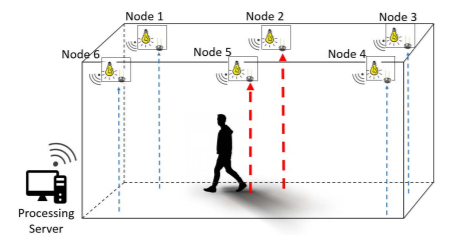
\includegraphics[width=90mm]{pics/lightspdceiling.png}
	\caption{Overview of the system set-up of "Activity sensing using ceiling photosensors" project \cite{Ceiling_PD}. In this specific situation node 2 and 5 detect shadow caused by the person in the room, while other nodes do not.}
\end{figure}

\section{Related visible light techniques}
A lot of projects make use of visible light, but in another way 

There is one other project in the VLC world that has nothing to do with human sensing. Zhao Tian \textit{et al} explores the idea of VLC with dark light, a VLC primitive that allows light-based communication to be sustained even when LEDs emit extremely-low luminance \cite{Dark_Light_Rises} \cite{Dark_VLC}. The communication works by generating high power, but short light pulses (500ns). These pulses are then used in a pulse position modulation scheme to achieve communication (1.8Kbps at 1.3m) with light while being nearly invisible to the end user.

\cite{Human_Sensing_Using_VLC}
